\documentclass[aspectratio=169,11pt]{beamer}

\usetheme{Madrid}
\usecolortheme{default}
\usefonttheme{professionalfonts}
\setbeamertemplate{navigation symbols}{}
\setbeamertemplate{blocks}[rounded][shadow=false]

\usepackage[T1]{fontenc}
\usepackage[utf8]{inputenc}
\usepackage{lmodern}
\usepackage{amsmath}
\usepackage{booktabs}
\usepackage{tabularx}
\usepackage{array}
\usepackage{graphicx}
\usepackage{tikz}
\usepackage{ragged2e}
\usepackage{xcolor}

\definecolor{AgroGreen}{HTML}{2F6B3B}
\definecolor{AgroLeaf}{HTML}{7FAE63}
\definecolor{AgroSoil}{HTML}{8C5A3C}
\definecolor{AgroCream}{HTML}{F7F3EA}
\definecolor{AgroInk}{HTML}{1E2A1F}
\definecolor{AgroGold}{HTML}{D9A441}

\setbeamercolor{normal text}{fg=AgroInk,bg=white}
\setbeamercolor{structure}{fg=AgroGreen}
\setbeamercolor{frametitle}{fg=white,bg=AgroGreen}
\setbeamercolor{title}{fg=white}
\setbeamercolor{subtitle}{fg=AgroCream}
\setbeamercolor{author}{fg=AgroCream}
\setbeamercolor{date}{fg=AgroCream}
\setbeamercolor{block title}{fg=white,bg=AgroGreen}
\setbeamercolor{block body}{fg=AgroInk,bg=AgroCream}
\setbeamercolor{itemize item}{fg=AgroGold}
\setbeamercolor{itemize subitem}{fg=AgroLeaf}

\setbeamerfont{title}{series=\bfseries,size=\Large}
\setbeamerfont{frametitle}{series=\bfseries,size=\large}

\newcommand{\accentline}{\textcolor{AgroGold}{\rule{\linewidth}{1.1pt}}}

\title{AgroVision}
\subtitle{A Multimodal Agricultural Assistant for Text, Image, and Audio Queries}
\author{Project Prototype Presentation}
\date{15-minute Beamer Prototype}

\begin{document}

{
\setbeamertemplate{background}{

\begin{tikzpicture}[remember picture,overlay]
\fill[AgroGreen] (current page.south west) rectangle (current page.north east);
\fill[AgroLeaf, opacity=0.18] (current page.north east) circle [radius=2.8cm];
\fill[AgroGold, opacity=0.10] (current page.south west) circle [radius=3.2cm];
\end{tikzpicture}
}
\begin{frame}[plain]
    \titlepage
    \vspace{-0.6em}
    {\color{AgroCream}\small
    Platform assumption for this prototype:
    users can submit \textbf{image + text}, \textbf{text only}, or \textbf{audio only} queries.}
\end{frame}
}

\begin{frame}{Talk Roadmap}
\begin{itemize}
    \item Problem and product vision
    \item Platform experience and supported modalities
    \item Model architecture and training pipeline
    \item Datasets, results, and example output
    \item Limitations and next steps
\end{itemize}
\end{frame}

\begin{frame}{Problem We Are Solving}
\begin{block}{Core Need}
Farmers, students, and agronomy practitioners need quick crop-health guidance without always typing long technical descriptions.
\end{block}
\vspace{0.4em}
\begin{itemize}
    \item Disease recognition often depends on both \textbf{visual cues} and \textbf{domain knowledge}.
    \item Many users prefer different input modes depending on context:
    \begin{itemize}
        \item field image + typed question,
        \item text-only agronomy question,
        \item spoken question when hands are busy.
    \end{itemize}
    \item The goal is one assistant that can unify these entry points.
\end{itemize}
\end{frame}

\begin{frame}{Platform Vision}
\begin{columns}[T]
    \column{0.48\textwidth}
    \begin{block}{Supported User Flows}
    \begin{itemize}
        \item \textbf{Image + text}: ``What disease is visible and how severe is it?''
        \item \textbf{Text only}: ``How much phosphorus per hectare should I apply to wheat?''
        \item \textbf{Audio only}: spoken agronomy question captured by the platform
    \end{itemize}
    \end{block}

    \column{0.48\textwidth}
    \begin{block}{System Behavior}
    \begin{itemize}
        \item Audio is transcribed to text in the platform layer.
        \item Text and transcribed audio use the same language-reasoning path.
        \item Image + text uses the full multimodal path.
    \end{itemize}
    \end{block}
\end{columns}
\vspace{0.5em}
\accentline
\vspace{0.2em}
\small The repository implements the language and vision-language core; this presentation adds audio as a product-level input channel.
\end{frame}

\begin{frame}{What the Repository Actually Implements}
\begin{itemize}
    \item \textbf{Base language model}: \texttt{Qwen/Qwen2.5-0.5B-Instruct}
    \item \textbf{Vision encoder}: \texttt{openai/clip-vit-large-patch14}
    \item \textbf{Alignment module}: a two-layer \textbf{MLP projector}
    \item \textbf{Adaptation}: agriculture LoRA + visual LoRA
    \item \textbf{Run context from the HTML report}: Google Colab T4 GPU
    \item \textbf{Inference paths}:
    \begin{itemize}
        \item \texttt{generate\_text\_only(...)}
        \item image-conditioned generation using all visual patches
    \end{itemize}
    \item \textbf{Frontend/backend references in README}: Streamlit frontend and FastAPI inference server
\end{itemize}
\vspace{0.3em}
\begin{alertblock}{Important correction}
The disease image data used for multimodal training is \textbf{PlantVillage}, not the local \texttt{/dataset} folder.
\end{alertblock}
\end{frame}

\begin{frame}{End-to-End System Architecture}
\small
\begin{center}
\begin{tabular}{>{\RaggedRight\arraybackslash}p{0.18\linewidth} >{\centering\arraybackslash}p{0.06\linewidth} >{\RaggedRight\arraybackslash}p{0.66\linewidth}}
Image input & $\rightarrow$ & CLIP ViT-Large/14 encodes the crop image into patch embeddings \\
Patch tokens & $\rightarrow$ & 256 spatial tokens are kept; the CLS token is dropped \\
Projector & $\rightarrow$ & MLP maps vision embeddings into the LLM hidden space \\
Language input & $\rightarrow$ & User text or audio transcript is tokenized with Qwen2.5 \\
Fusion & $\rightarrow$ & Visual embeddings are concatenated with text embeddings \\
LLM + LoRA & $\rightarrow$ & Agriculture LoRA provides domain knowledge; visual LoRA improves multimodal reasoning \\
Output & $\rightarrow$ & Diagnosis, severity estimate, management advice, or general agronomy answer
\end{tabular}
\end{center}
\vspace{0.4em}
\begin{block}{Key design choice}
The code keeps \textbf{all 256 image patches}, allowing the LLM to attend to lesion patterns, color changes, and texture regions rather than a single pooled visual token.
\end{block}
\end{frame}

\begin{frame}{Training Pipeline in Three Steps}
\begin{enumerate}
    \item \textbf{Text-only domain adaptation}
    \begin{itemize}
        \item Fine-tune a LoRA on agricultural QA text.
        \item Dataset used in code: \texttt{KisanVaani/agriculture-qa-english-only}.
    \end{itemize}
    \item \textbf{Stage 1 visual alignment}
    \begin{itemize}
        \item Freeze ViT and LLM.
        \item Train only the projector on image-caption pairs.
    \end{itemize}
    \item \textbf{Stage 2 multimodal adaptation}
    \begin{itemize}
        \item Keep ViT frozen.
        \item Train projector + new visual LoRA on VQA triplets.
    \end{itemize}
\end{enumerate}
\vspace{0.4em}
\begin{block}{Why this works}
The pipeline first teaches the model agricultural language, then teaches image tokens to ``speak'' the LLM embedding space, then tunes multimodal reasoning.
\end{block}
\end{frame}

\begin{frame}{Datasets Used}
\begin{columns}[T]
    \column{0.52\textwidth}
    \begin{block}{Text Training Data}
    \begin{itemize}
        \item Source: \texttt{KisanVaani/agriculture-qa-english-only}
        \item Processed rows mentioned in logs: \textbf{22,574 usable}
        \item Training subset written to JSONL: \textbf{8,000 rows}
        \item Stage 0 setup: \textbf{450 max steps}, effective batch size 16
    \end{itemize}
    \end{block}

    \column{0.44\textwidth}
    \begin{block}{Vision-Language Data}
    \begin{itemize}
        \item Source for disease images: \textbf{PlantVillage}
        \item Stage 1: \textbf{1,000} generated image-caption pairs
        \item Stage 2: \textbf{1,000} generated VQA triplets
        \item \textbf{4} QA pairs used per image from 5 templates
        \item Notebook examples use PlantVillage apple disease images
    \end{itemize}
    \end{block}
\end{columns}
\vspace{0.4em}
\begin{alertblock}{Dataset clarification}
For the presentation, the correct multimodal dataset statement is:
\textbf{``We use PlantVillage for visual disease learning, not the local /dataset directory.''}
\end{alertblock}
\end{frame}

\begin{frame}{Generated Supervision Strategy}
\begin{itemize}
    \item \textbf{Stage 1 captions} are automatically produced from class labels such as \texttt{Tomato\_\_\_Early\_blight}.
    \item \textbf{Stage 2 VQA} creates reviewable question-answer pairs like:
    \begin{itemize}
        \item disease identification,
        \item severity estimation,
        \item visual evidence,
        \item management advice,
        \item prevention.
    \end{itemize}
    \item This makes training feasible even when manual multimodal annotations are limited.
\end{itemize}
\vspace{0.4em}
\begin{block}{Practical note}
The repo explicitly notes that the generated VQA answers are template-based and should be manually reviewed before production use.
\end{block}
\end{frame}

\begin{frame}{Training Snapshot}
\small
\begin{center}
\begin{tabularx}{\linewidth}{lccc}
\toprule
\textbf{Phase} & \textbf{Epoch / Run} & \textbf{Metric} & \textbf{Value} \\
\midrule
Text LoRA & final run & train loss & 0.9349 \\
Projector Stage 1 & epoch 1 & avg loss & 0.5500 \\
Projector Stage 1 & epoch 2 & avg loss & 0.0347 \\
Projector Stage 1 & epoch 3 & avg loss & 0.0090 \\
Stage 2 multimodal & epoch 1 & avg loss & 0.3996 \\
Stage 2 multimodal & epoch 2 & avg loss & 0.0994 \\
Stage 2 multimodal & epoch 3 & avg loss & 0.0141 \\
\bottomrule
\end{tabularx}
\end{center}
\vspace{0.4em}
\begin{itemize}
    \item HTML report summary: \textbf{8.8M trainable parameters}, about \textbf{1.75\%} of a 502M-parameter model.
    \item Stage 0 runtime reported: \textbf{1007 seconds} with about \textbf{7.15 samples/s}.
\end{itemize}
\end{frame}

\begin{frame}{Stage 0 Plot: LLM Fine-Tuning}
\begin{columns}[T]
    \column{0.62\textwidth}
    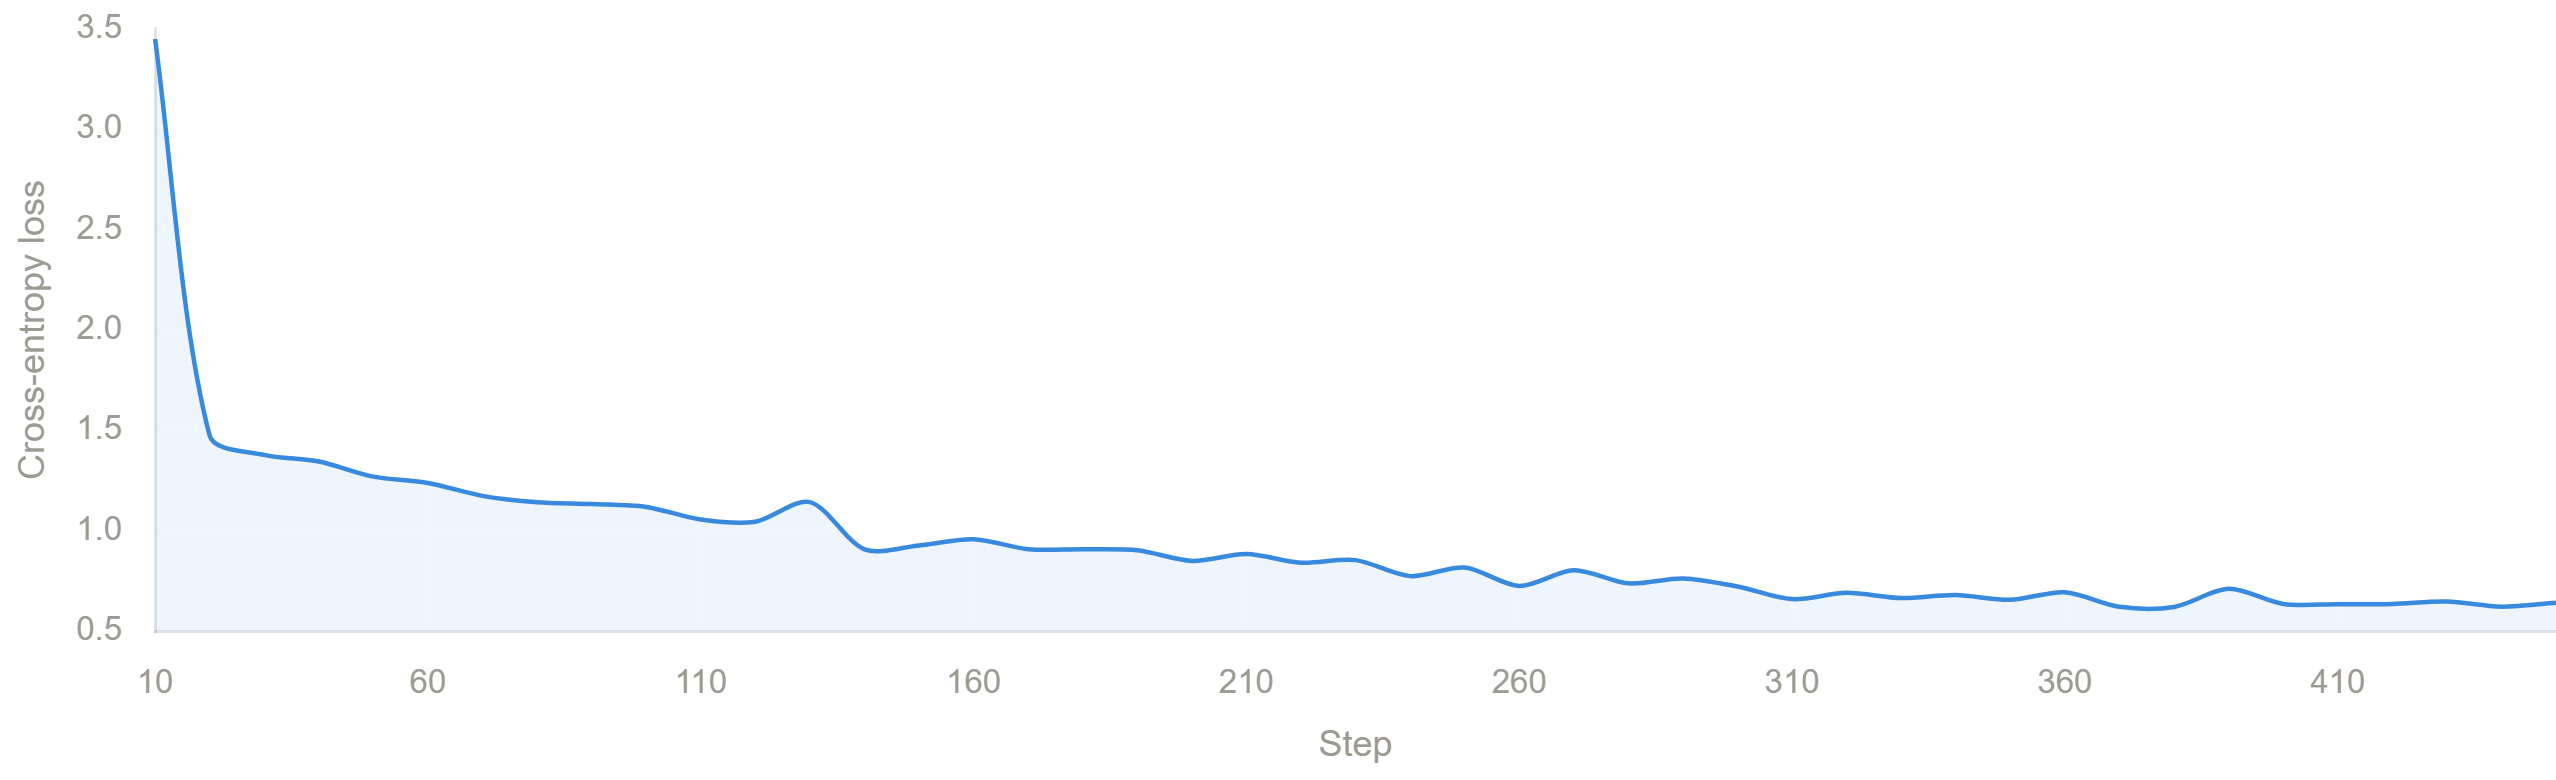
\includegraphics[width=\linewidth,height=0.72\textheight,keepaspectratio]{plots/LLM fine-tuning loss curve.png}

    \column{0.34\textwidth}
    \small
    \begin{block}{What changed}
    \begin{itemize}
        \item LoRA trained on \textbf{8,000} agricultural QA samples
        \item Sharp early drop, then steady convergence
        \item Final logged train loss: \textbf{0.9349}
    \end{itemize}
    \end{block}
    \begin{block}{Reading}
    The HTML report notes the curve falls fast in the first 100 steps, then continues decreasing through the 450-step run.
    \end{block}
\end{columns}
\end{frame}

\begin{frame}{Stage 1 Plot: Caption Alignment}
\begin{columns}[T]
    \column{0.62\textwidth}
    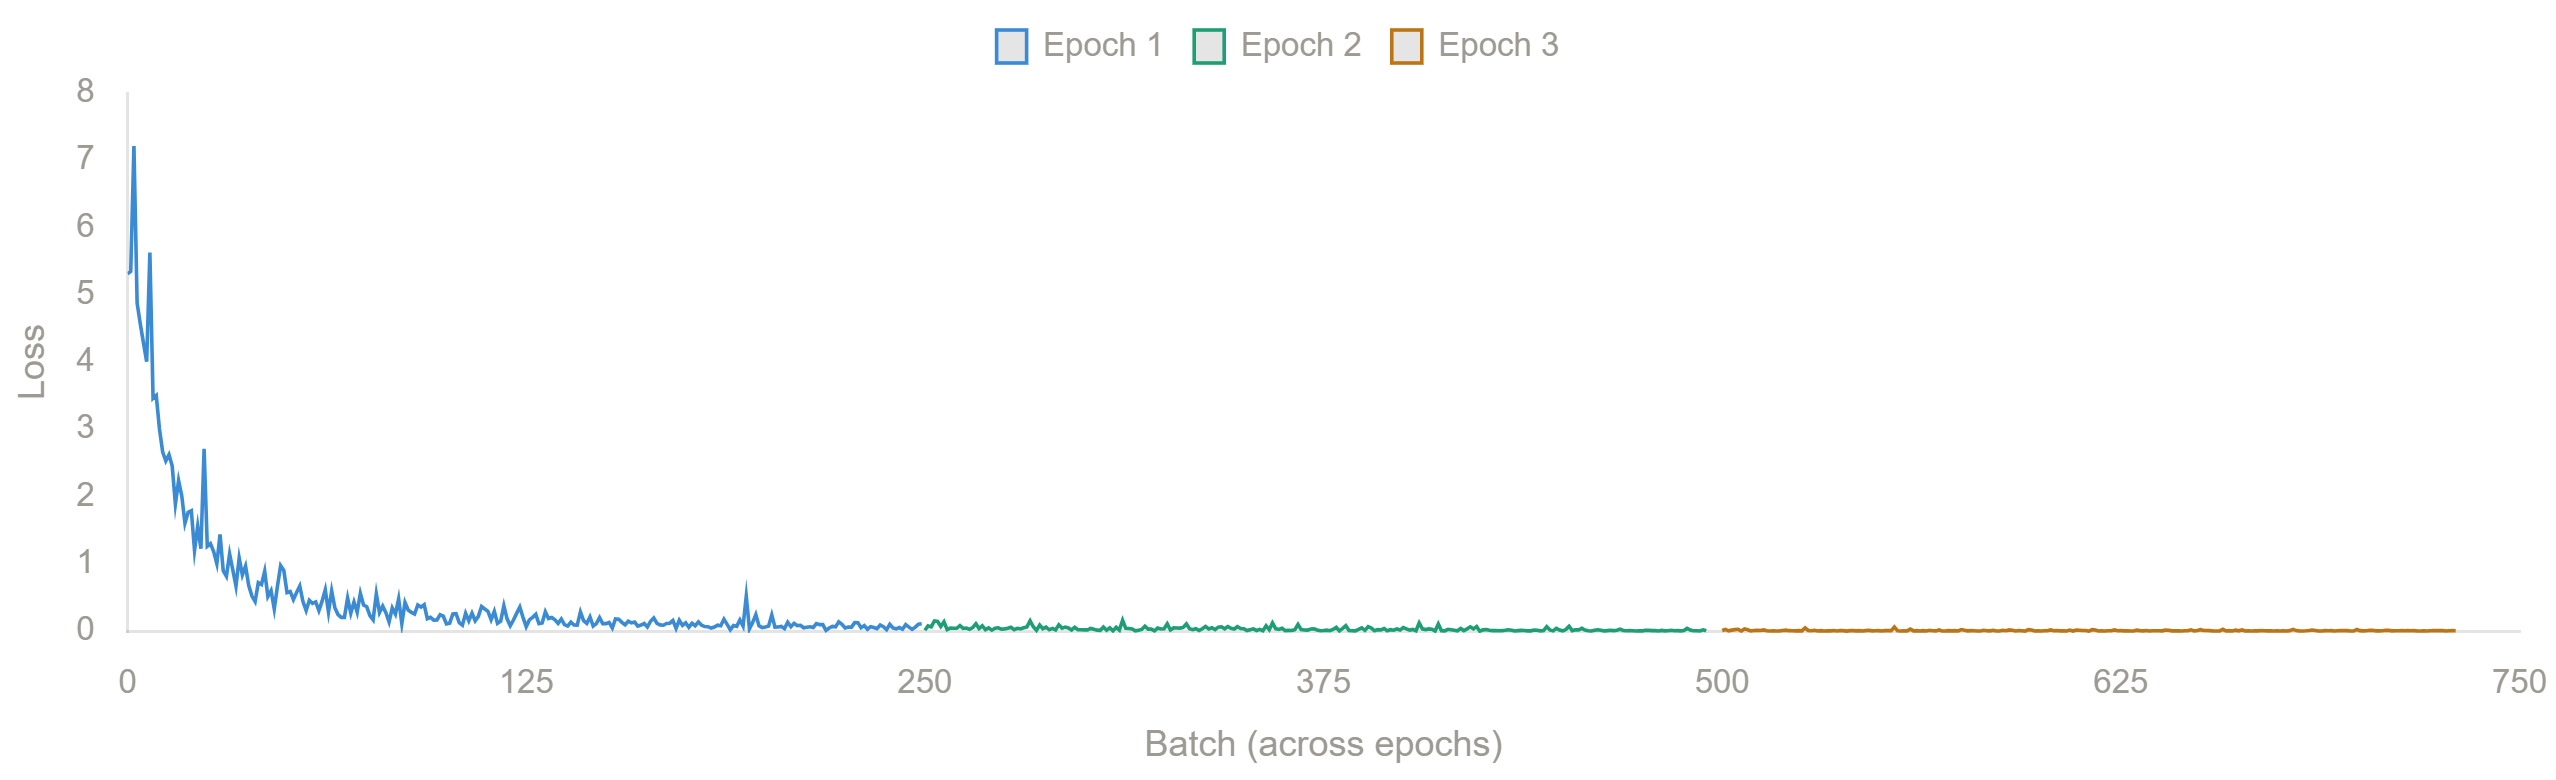
\includegraphics[width=\linewidth,height=0.72\textheight,keepaspectratio]{plots/Projector loss curves (caption alignment).png}

    \column{0.34\textwidth}
    \small
    \begin{block}{Stage 1}
    \begin{itemize}
        \item Frozen: ViT + LLM
        \item Trained: projector only
        \item Data: \textbf{1,000} caption pairs from PlantVillage
        \item Final loss: \textbf{0.0090}
    \end{itemize}
    \end{block}
    \begin{block}{Interpretation}
    This is the cleanest convergence phase in the pipeline and shows that the projector successfully learns the vision-to-language bridge.
    \end{block}
\end{columns}
\end{frame}

\begin{frame}{Stage 2 Plot: VQA Alignment}
\begin{columns}[T]
    \column{0.62\textwidth}
    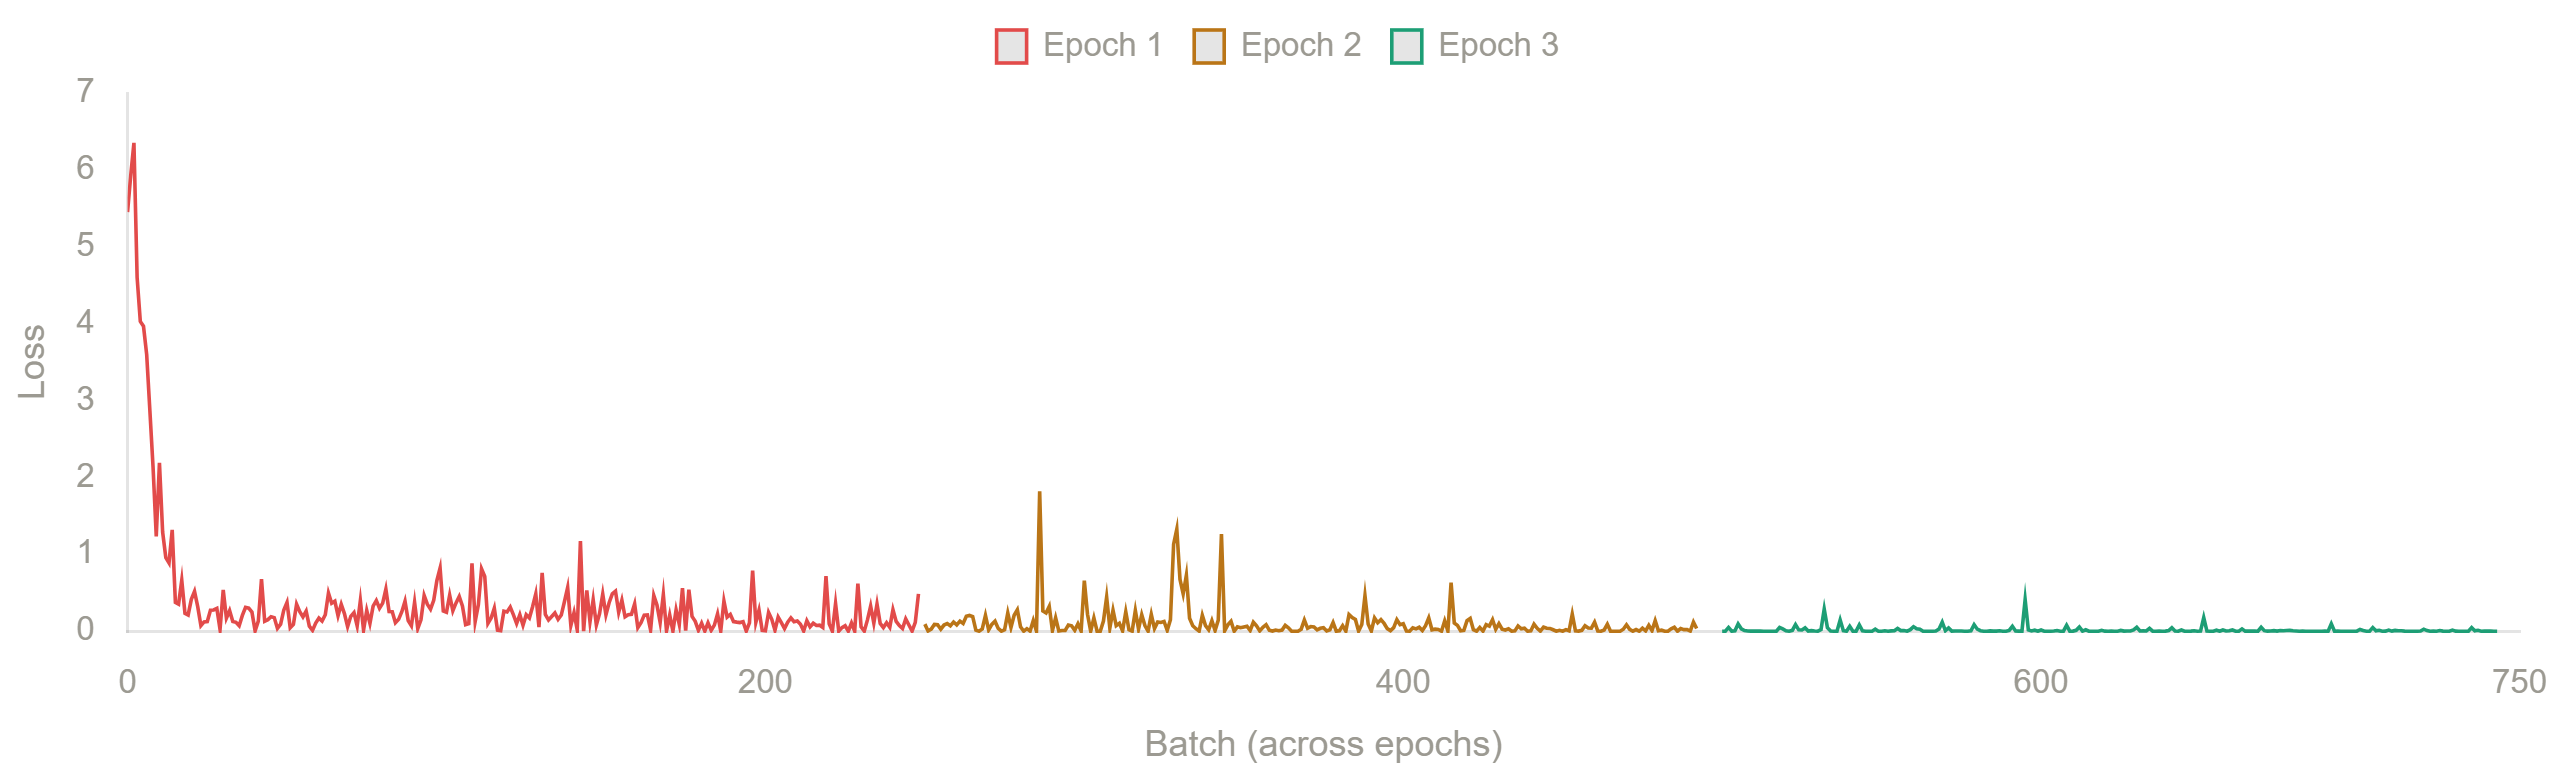
\includegraphics[width=\linewidth,height=0.72\textheight,keepaspectratio]{plots/Projectorlosscurves_(VQA alignment).png}

    \column{0.34\textwidth}
    \small
    \begin{block}{Stage 2}
    \begin{itemize}
        \item Frozen: ViT + LLM backbone
        \item Trained: projector + visual LoRA
        \item Data: \textbf{1,000} PlantVillage VQA triplets
        \item Final loss: \textbf{0.0141}
    \end{itemize}
    \end{block}
    \begin{block}{Interpretation}
    The first epoch is noisier because VQA is harder than captioning, but the run still converges cleanly by epoch 3.
    \end{block}
\end{columns}
\end{frame}

\begin{frame}{Example Inference Story}
\begin{block}{Text-only example from the report}
\small
Query: ``How much phosphorus per hectare should I apply to wheat?''
\end{block}
\vspace{0.3em}
\begin{block}{Multimodal example from the report}
\small
Input image: infected apple leaf from the PlantVillage \texttt{Apple\_\_\_Apple\_scab} class \\
Prompt: ``What disease is visible and how severe is it?''
\end{block}
\vspace{0.4em}
\begin{itemize}
    \item The reported output identifies visible spots and lesions and provides disease-aware reasoning.
    \item The new HTML report also highlights an important limitation: the model recognizes disease symptoms but still hallucinates some pathogen details.
    \item This demonstrates the shift from pure agronomy QA to image-grounded crop diagnosis, while still leaving room for factual calibration.
\end{itemize}
\end{frame}

\begin{frame}{How Audio Fits the Platform}
\begin{columns}[T]
    \column{0.49\textwidth}
    \begin{block}{User Experience}
    \begin{itemize}
        \item Farmer speaks a question in the field.
        \item Platform records audio and runs speech-to-text.
        \item Transcript is sent to the same assistant.
    \end{itemize}
    \end{block}

    \column{0.49\textwidth}
    \begin{block}{System Mapping}
    \begin{itemize}
        \item Audio only $\Rightarrow$ ASR transcript $\Rightarrow$ text-only inference
        \item Image + text stays multimodal
        \item Future extension: image + audio can become image + transcript
    \end{itemize}
    \end{block}
\end{columns}
\vspace{0.4em}
\begin{alertblock}{Message for the audience}
Audio support expands accessibility without changing the core reasoning backbone: it is a new input interface, not a separate model family.
\end{alertblock}
\end{frame}

\begin{frame}{Why This Design Is Practical}
\begin{itemize}
    \item \textbf{Efficient}: LoRA keeps training lightweight relative to full fine-tuning.
    \item \textbf{Modular}: vision encoder remains frozen; only projector and adapters are trained.
    \item \textbf{Accessible}: one platform supports typed, visual, and spoken interaction.
    \item \textbf{Deployable}: repository references Streamlit frontend and API-based serving.
    \item \textbf{Domain-focused}: agricultural QA knowledge is injected before multimodal training.
\end{itemize}
\end{frame}

\begin{frame}{Current Limitations}
\begin{itemize}
    \item Multimodal supervision is partly template-generated, so linguistic diversity is limited.
    \item PlantVillage is curated and clean; field images in real farms may be harder.
    \item The HTML report notes Stage 0 stops at about \textbf{0.9 epochs}, so the language adapter has not yet fully covered the full text dataset.
    \item The repository shows some documentation drift between README and code, so the implementation snapshot should be based on the latest report and scripts.
    \item Audio is presented here as a working platform feature layered on top of the repository core, not as a separately trained speech model in this repo.
\end{itemize}
\end{frame}

\begin{frame}{Next Steps}
\begin{enumerate}
    \item Connect live ASR to the deployed frontend for real spoken queries.
    \item Increase Stage 0 training beyond 450 steps and add validation-based early stopping.
    \item Validate on real field images beyond PlantVillage.
    \item Add multilingual prompts and speech support.
    \item Replace template-generated captions and VQA pairs with expert-reviewed supervision.
    \item Consider a larger backbone such as \texttt{Qwen2.5-1.5B} for stronger reasoning.
\end{enumerate}
\end{frame}

\begin{frame}{Takeaway}
\begin{block}{Final Message}
AgroVision is a strong prototype of a \textbf{multimodal agricultural assistant}:
\begin{itemize}
    \item trained first on agricultural text knowledge,
    \item aligned to \textbf{PlantVillage} crop-disease images,
    \item and presented as a platform that supports \textbf{text}, \textbf{image + text}, and \textbf{audio} interaction.
\end{itemize}
\end{block}
\vspace{0.5em}
\centering
\Large\textcolor{AgroGreen}{One assistant, multiple field-friendly ways to ask for help.}
\end{frame}

\end{document}
